\documentclass[11pt]{article}
\usepackage[margin=1in]{geometry}
\usepackage{graphicx}
\begin{document}
\section*{R91 bidirectional rank-32 RR transport}
The single frozen R91 attempt checked all 32 normalized R50 generators in
both rational diamond directions. The exact native gate passed 64 column
products and 64 corrupted-coordinate controls. Independent replay from a
fresh S3 readback checked both full products, 64 columns and 2,048
polynomial module coordinates in an ideal-free coefficient field.

\begin{center}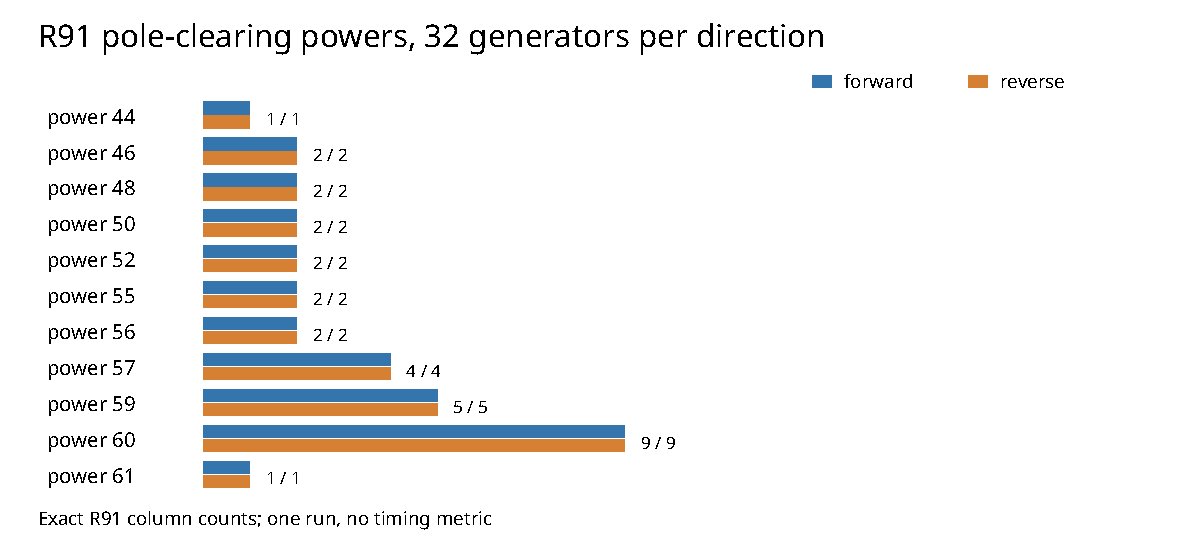
\includegraphics[width=\textwidth]{power-histogram.pdf}\end{center}

The first pole-clearing powers range from 44 to 61 in each direction.
The forward and reverse 32-value sequences coincide; one generator in
each direction attains the bound 61. These are exact counts, not timings.
Source revision \texttt{7ff259920}; seed 91; one native Singular/FLINT
thread; 4 GiB virtual-memory cap; 1200-second timeout. All 18 raw members
passed fresh-readback hashes. Earlier polynomial-ring replay probes failed
because exported power vectors include rational coefficients; the
corrected ideal-free F2(u) replay passes. The Lean module proves only the
conditional integer pole inequalities. Proper boundary normalization and
the modular-factor action remain the next constructions.
\end{document}
